%%% Econ712: Macroeconomics I
%%% Fall 2020
%%% Danny Edgel
%%%
% Due on Canvas Thursday October 8, 11:59pm Central Time
%%%

%%%
%							PREAMBLE
%%%

\documentclass{article}

%%% declare packages
\usepackage{amsmath}
\usepackage{amssymb}
\usepackage{array}
\usepackage{bm}
\usepackage{changepage}
\usepackage{centernot}
\usepackage{graphicx}
\usepackage{fancyhdr}
	\fancyhf{} % sets both header and footer to nothing
	\renewcommand{\headrulewidth}{0pt}
    \rfoot{Edgel, \thepage}
    \pagestyle{fancy}
	
%%% define shortcuts for set notation
\newcommand{\N}{\mathbb{N}}
\newcommand{\Z}{\mathbb{Z}}
\newcommand{\R}{\mathbb{R}}
\newcommand{\Q}{\mathbb{Q}}
\newcommand{\lmt}{\underset{x\rightarrow\infty}{\text{lim }}}
\newcommand{\neglmt}{\underset{x\rightarrow-\infty}{\text{lim }}}
\newcommand{\zerolmt}{\underset{x\rightarrow 0}{\text{lim }}}
\newcommand{\loge}[1]{\text{ln}\left(#1\right)}
\newcommand{\usmax}[1]{\underset{\{#1\}}{\text{max }}}
\newcommand{\Mt}{M_{t+1}^t}
\renewcommand{\L}{\mathcal{L}}
\newcommand{\olq}{\overline{q}}

%%% define column vector command (from Michael Nattinger)
\newcount\colveccount
\newcommand*\colvec[1]{
        \global\colveccount#1
        \begin{pmatrix}
        \colvecnext
}
\def\colvecnext#1{
        #1
        \global\advance\colveccount-1
        \ifnum\colveccount>0
                \\
                \expandafter\colvecnext
        \else
                \end{pmatrix}
        \fi
}

%%% define function for drawing matrix augmentation lines
\newcommand\aug{\fboxsep=-\fboxrule\!\!\!\fbox{\strut}\!\!\!}

\makeatletter
\let\amsmath@bigm\bigm

\renewcommand{\bigm}[1]{%
  \ifcsname fenced@\string#1\endcsname
    \expandafter\@firstoftwo
  \else
    \expandafter\@secondoftwo
  \fi
  {\expandafter\amsmath@bigm\csname fenced@\string#1\endcsname}%
  {\amsmath@bigm#1}%
}


%________________________________________________________________%

\begin{document}

\title{	Problem Set \#5 }
\author{ 	Danny Edgel 					\\ 
			Econ 712: Macroeconomics I		\\
			Fall 2020						\\
		}
\maketitle\thispagestyle{empty}

%%%________________________________________________________________%%%

\noindent\textit{Collaborated with Sarah Bass, Emily Case, Michael Nattinger, and Alex Von Hafften}


%%%________________________________________________________________%%%

\section*{Question 2.1}
The individual labor supply curve is derived by solving the worker's recursive problem:
\[
	V_j(k) = \usmax{k',\ell_j}\left\{u_j^W(c,\ell) + \beta V_j(k') \right\}\text{ s.t } c=(1-\tau)e_j w\ell_j + (1+r)k - k'
\]
Where:
\[
	u_j^W = \frac{\left(c_j^\gamma(1-\ell_j)^{1-\gamma}\right)^{1-\sigma}}{1-\sigma}
\]
Letting $\ell_j=l$ and taking the first order condition with respect to $l$ (after substituting the right side of the budget constraint for $c$) allows us to solve for the individual labor supply:
\[
	\frac{\partial V_j(k)}{\partial l} = 
	\frac{\partial}{\partial l} \left[ \frac{\left([(1-\tau)e_jwl+(1+r)k-k']^\gamma(1-l)^{1-\gamma}\right)^{1-\sigma}}{1-\sigma}\right] = 0
\]
\begin{align*}
	& 0 = \left([(1-\tau)e_jwl+(1+r)k-k']^\gamma(1-l)^{1-\gamma}\right)^{-\sigma} \\
	&\left[\gamma\left((1-\tau)e_jwl+(1+r)k-k'\right)^{\gamma-1}(1-\tau)e_jw(1-l)^{1-\gamma} 
	-(1-\gamma)((1-\tau)e_jwl+(1+r)k-k')^\gamma(1-l)^{-\gamma}\right] 
\end{align*}
\[
	[(1-\tau)e_jwl+(1+r)k-k']^\gamma
	\left[\frac{\gamma(1-\tau)e_jw(1-l)^{1-\gamma}}{(1-\tau)e_jwl+(1+r)k-k'} - \frac{1-\gamma}{(1-l)^\gamma}\right] 
	= 0
\]
\begin{align*}
	\gamma(1-\tau)e_jw(1-l) 					&= (1-\gamma)[(1-\tau)E_jwl+(1+r)k-k' 				\\
	\gamma(1-\tau)e_jw-(1-\gamma)[(1+r)k+k'] 	&= (1-\gamma)(1-\tau)we_jl+\gamma(1-\tau)e_jwl 		\\
	\gamma(1-\tau)e_jw-(1-\gamma)[(1+r)k+k'] 	&= (1-\tau)e_jwl
\end{align*}
\[
	l = \frac{\gamma(1-\tau)e_jw-(1-\gamma)[(1+r)k+k']}{(1-\tau)e_jw}
\]


%%%________________________________________________________________%%%

\section*{Question 2.2}

Please see the code provided, ``edgel\_ps5.R", for my omputations. A Matlab version is also available, but the plots provided below were generated by the R code.

%%%________________________________________________________________%%%

\section*{Question 2.3}

In each run of the while loop, capital and labor are calculated, and the loop gives the model 100 iterations to converge within a specified level of tolerance (in this case, 0.001). If both labor and capital change from one period to another within the tolerance level, the loop finishes, presuming that labor and capital have converged to their steady state.\footnote{Convergence to the steady state has indeed occurred if the initial guess was close enough to the steady state.} Prior to the first for loop, the current period's prices are calculated according to the period's labor and capital levels, which are then used to calculate the oldest agents' consumption and utility level. The first for loop iterates through each retired age cohort and determines its agents' optimal level of capital, consumption, and utility by maximizing the bellman equation using the capital levels from the capital grid. \\

The next for loop repeats the methodology of the retired cohorts loop for working cohorts. However, in this loop, labor supply is determined using the individual labor supply curve that was derived in question 2.1. After using capital and savings to determine labor supply, consumption and utility are calculated, and the optimal savings can be derived by maximizing the bellman equation. \\

Each cohort loop fills in an array that provides optimal capital savings and, for working generations, optimal labor for each capital level in the capital grid. Following each cohort loop, each generation's actual capital and labor are determined by starting with the first generation's capital endowment, then, in the final for loop, iterating forward through each age and calculating capital and labor at that age. Following that loop, labor and capital are re-calculated by multiplying these generation-specific labor and capital values by the relative weight of each generation, then updating the steady-state guess.


%%%________________________________________________________________%%%

\section*{Question 2.4}
The plot below displays the value function against $k$ of a retired agent at age 50, assuming social security is in place. It is clearly both increasing and concave.
\begin{center}
	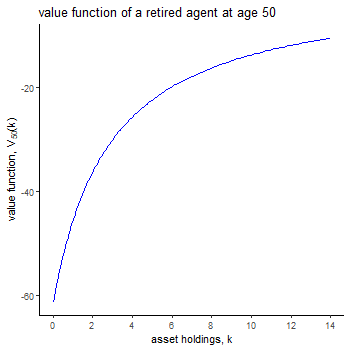
\includegraphics[scale = .65]{value_ss.png}
\end{center}
The next plot displays current-period $k$ (x-axis) against savings, $k'$ (y-axis), with the 45$^{\circ}$ line for comparison, for a working agent at age 20. This was generated using the same model specifications as the value function displayed above. Given its near-unity with the 45$^{\circ}$ line, its shape is not as obvious as that of the value function. However, it is still concave and increasing, with net savings ($k'-k$) decreasing as $k$ increases.
\begin{center}
	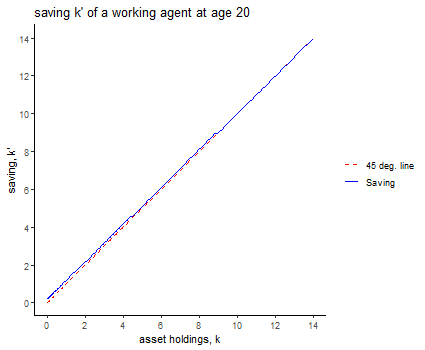
\includegraphics[scale = .65]{savingk_ss.png}
\end{center}

%%%________________________________________________________________%%%

\section*{Question 2.5}

The results of the model are displayed in the table below.
\begin{center}
	\begin{tabular}{r|c c}
									&	\multicolumn{2}{c}{Benchmark model}	 				\\
									& with SS 		& without SS			 				\\
		\hline\hline				&				&										\\
		capital $K$					& 2.978			& 3.911									\\
		labor $L$					& 0.351			& 0.369									\\
		wage $w$					& 1.382			& 1.498									\\
		interest $r$				& 0.032			& 0.019									\\
		pension benefit $b$			& 0.219			& 0.000									\\
		newborn welfare $V_1(k_1)$	& -54.613		& -52.764								\\
		aggregate welfare $W$		& -35.069		& -36.034
	\end{tabular}
\end{center}

\begin{enumerate}
	\item The implicit return on social security is equal to the population growth rate of $0.011$, and the interest rate in the social security equilibrium, 0.032, is higher than that implicit return. Therefore, this economy is dynamically efficient.
	\item New equilibrium values of aggregate capital and labor supply are displayed in the table above. The wealth profiles of each age group in each scenario are diplayed in the plot below. The fact that wealth peaks at the age of retirement in both scenarios is intuitive because agents save in each working period, then consume their wealth throughout retirement. It is also intuitive that agents have less wealth at each age\footnote{It appears that agents have slightly more wealth around age 29-37 in the social security scenario. This gap is negligible, however.} in the social security scenario, and that the gap between the scenarios shinks during retirement. In the no social security scenario, agents will only consume the value of their wealth during retirement, so in order to maximize their lifetime utility, they must save more. In the social security scenario, they can achieve that same level of utility with less wealth because they can consume off of pension benefits during retirement. Therefore, in their working years, they consume more and/or take more liesure time and thus save less.
		\begin{center}
			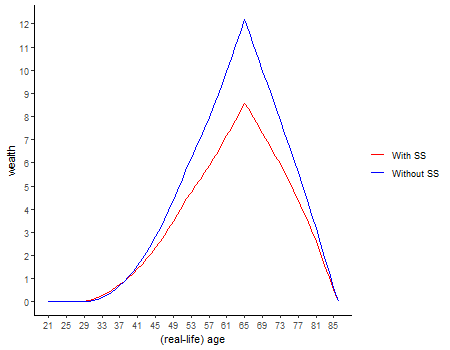
\includegraphics[scale = .65]{wealth.png}
		\end{center}
		In the no social security scenario, newborn welfare is higher than in the social security scenario. Therefore, a newborn generation would prefer to start in the steady state without social security. However, Aggregate welfare is higher in the social security steady state, so a reform that ends social security would not be supported by majority voting.
\end{enumerate}


%%%________________________________________________________________%%%


\end{document}












